% Options for packages loaded elsewhere
\PassOptionsToPackage{unicode}{hyperref}
\PassOptionsToPackage{hyphens}{url}
%
\documentclass[
]{article}
\usepackage{amsmath,amssymb}
\usepackage{lmodern}
\usepackage{iftex}
\ifPDFTeX
  \usepackage[T1]{fontenc}
  \usepackage[utf8]{inputenc}
  \usepackage{textcomp} % provide euro and other symbols
\else % if luatex or xetex
  \usepackage{unicode-math}
  \defaultfontfeatures{Scale=MatchLowercase}
  \defaultfontfeatures[\rmfamily]{Ligatures=TeX,Scale=1}
\fi
% Use upquote if available, for straight quotes in verbatim environments
\IfFileExists{upquote.sty}{\usepackage{upquote}}{}
\IfFileExists{microtype.sty}{% use microtype if available
  \usepackage[]{microtype}
  \UseMicrotypeSet[protrusion]{basicmath} % disable protrusion for tt fonts
}{}
\makeatletter
\@ifundefined{KOMAClassName}{% if non-KOMA class
  \IfFileExists{parskip.sty}{%
    \usepackage{parskip}
  }{% else
    \setlength{\parindent}{0pt}
    \setlength{\parskip}{6pt plus 2pt minus 1pt}}
}{% if KOMA class
  \KOMAoptions{parskip=half}}
\makeatother
\usepackage{xcolor}
\usepackage[margin=1in]{geometry}
\usepackage{longtable,booktabs,array}
\usepackage{calc} % for calculating minipage widths
% Correct order of tables after \paragraph or \subparagraph
\usepackage{etoolbox}
\makeatletter
\patchcmd\longtable{\par}{\if@noskipsec\mbox{}\fi\par}{}{}
\makeatother
% Allow footnotes in longtable head/foot
\IfFileExists{footnotehyper.sty}{\usepackage{footnotehyper}}{\usepackage{footnote}}
\makesavenoteenv{longtable}
\usepackage{graphicx}
\makeatletter
\def\maxwidth{\ifdim\Gin@nat@width>\linewidth\linewidth\else\Gin@nat@width\fi}
\def\maxheight{\ifdim\Gin@nat@height>\textheight\textheight\else\Gin@nat@height\fi}
\makeatother
% Scale images if necessary, so that they will not overflow the page
% margins by default, and it is still possible to overwrite the defaults
% using explicit options in \includegraphics[width, height, ...]{}
\setkeys{Gin}{width=\maxwidth,height=\maxheight,keepaspectratio}
% Set default figure placement to htbp
\makeatletter
\def\fps@figure{htbp}
\makeatother
\setlength{\emergencystretch}{3em} % prevent overfull lines
\providecommand{\tightlist}{%
  \setlength{\itemsep}{0pt}\setlength{\parskip}{0pt}}
\setcounter{secnumdepth}{5}
\usepackage{booktabs}
\usepackage{longtable}
\usepackage{array}
\usepackage{multirow}
\usepackage{wrapfig}
\usepackage{float}
\usepackage{colortbl}
\usepackage{pdflscape}
\usepackage{tabu}
\usepackage{threeparttable}
\usepackage{threeparttablex}
\usepackage[normalem]{ulem}
\usepackage{makecell}
\usepackage{xcolor}
\ifLuaTeX
  \usepackage{selnolig}  % disable illegal ligatures
\fi
\IfFileExists{bookmark.sty}{\usepackage{bookmark}}{\usepackage{hyperref}}
\IfFileExists{xurl.sty}{\usepackage{xurl}}{} % add URL line breaks if available
\urlstyle{same} % disable monospaced font for URLs
\hypersetup{
  pdftitle={Final Report},
  pdfauthor={Russell and Frances},
  hidelinks,
  pdfcreator={LaTeX via pandoc}}

\title{Final Report}
\author{Russell and Frances}
\date{5th October 2022}

\begin{document}
\maketitle

{
\setcounter{tocdepth}{2}
\tableofcontents
}
\hypertarget{health-of-new-zealand-lakes}{%
\section{Health of New Zealand Lakes}\label{health-of-new-zealand-lakes}}

\hypertarget{introduction}{%
\subsection{Introduction}\label{introduction}}

We are Russell and Frances and we form Group 8. Below are our pictures as well as our contact details and ORCID ID numbers.

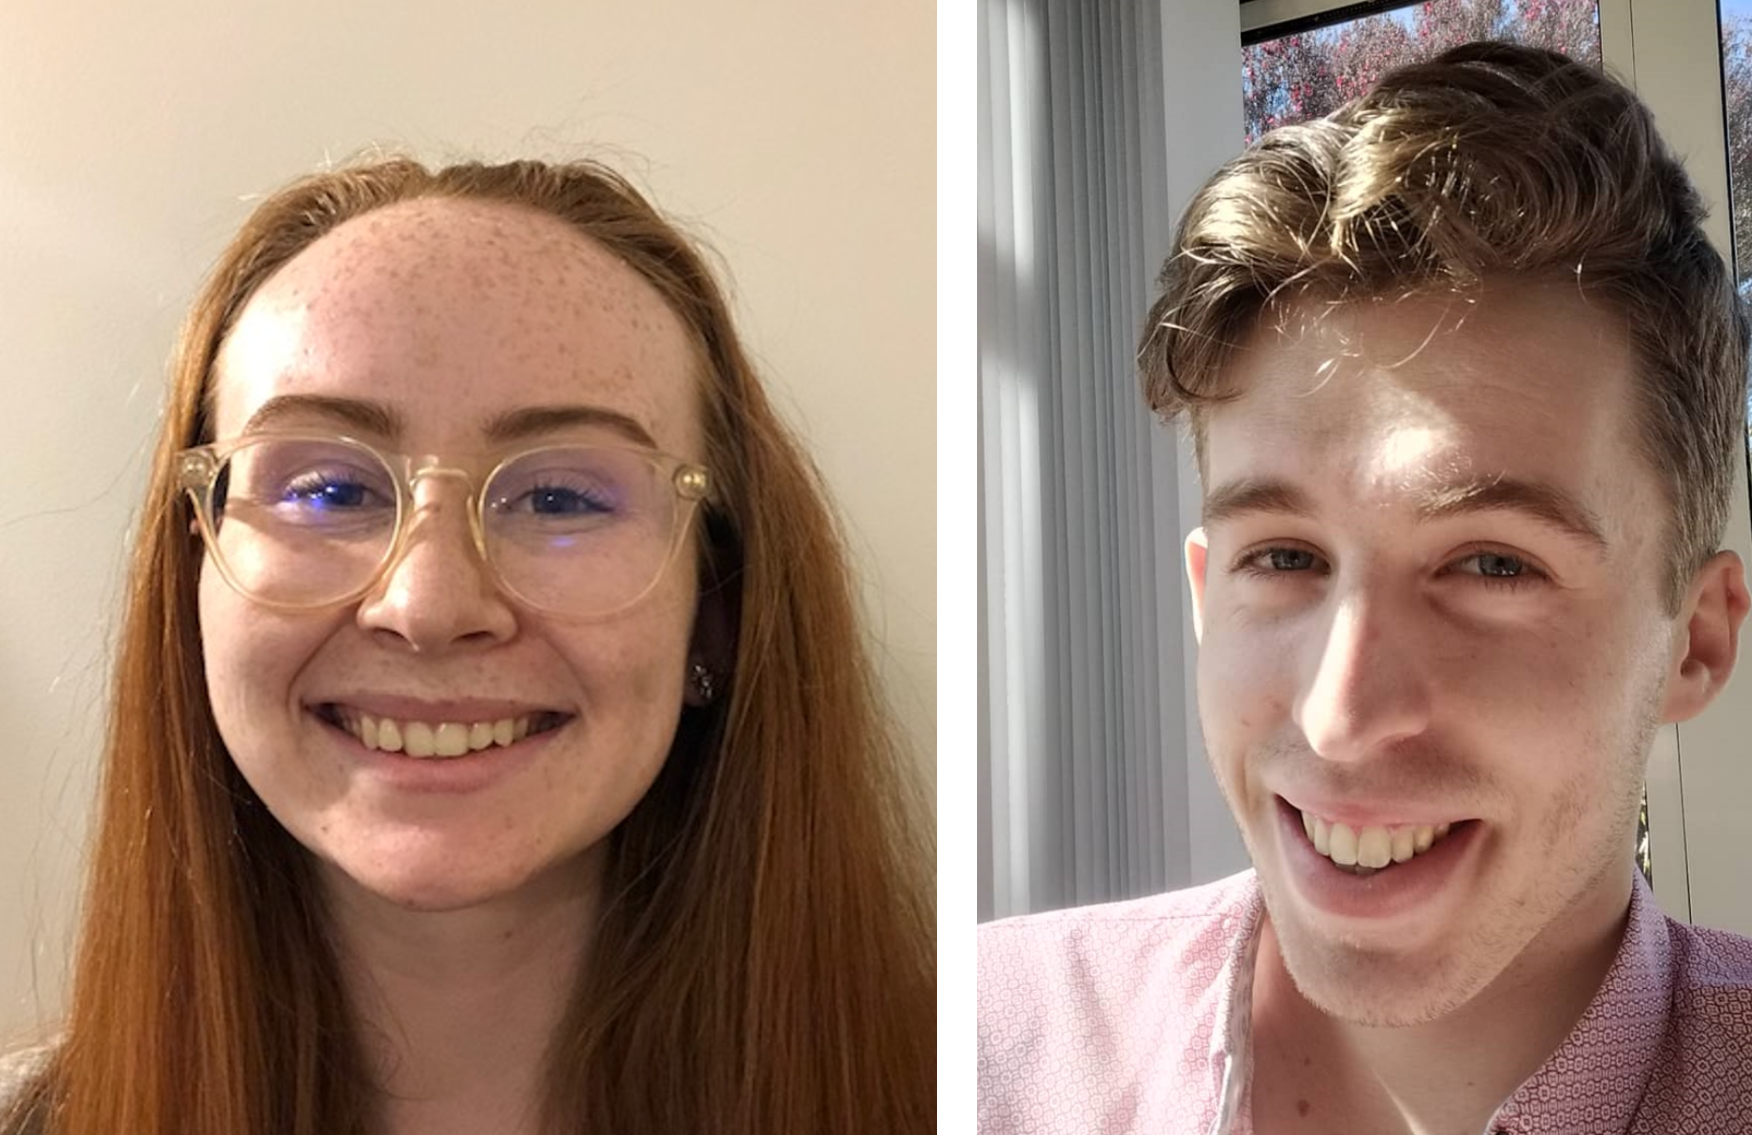
\includegraphics[width=0.4\linewidth,height=0.3\textheight]{../Presentations/Russell and Frances}

\textbf{Frances Smith}\\
email: \href{mailto:frances.j.smith.nz@gmail.com}{\nolinkurl{frances.j.smith.nz@gmail.com}}\\
ORCHID ID: 0000-0002-5168-3134

\textbf{Russell Syder}\\
email: \href{mailto:russellsyder@gmail.com}{\nolinkurl{russellsyder@gmail.com}}\\
ORCHID ID: 0000-0002-4582-5909

\hypertarget{introduction-to-our-data}{%
\subsubsection{Introduction to our data}\label{introduction-to-our-data}}

Our original dataset was extracted from Stats NZ.
\url{https://www.stats.govt.nz/indicators/modelled-lake-water-quality/}

We made some manipulations to the original dataset such as removing extraneous variables (like Date which was the same for every lake) or variables that we were not interested in. We also reshaped some aspects of the dataset so that the data would be easier to analyse. We checked for missing values; there were some for the categorical variables, which we dealt with as described below, but there were no missing values for the numerical variables so imputation was not necessary.

Our final dataset contains information from 3802 lakes (exceeding one hectare) in New Zealand measured across 22 variables. Of these 22 variables we selected 10 that we would use for further analysis. They are as follows:

\emph{Ammoniacal Nitrogen} is a form of nitrogen that supports algae and plant growth, but in large concentrations can be toxic to aquatic life. This is measured in milligrams per litre. The national bottom line for this measure is 1.3mg/L, which none of the observations exceed. It acts as as measure of toxicity.

\emph{Chlorophyll-A} is an organic molecule found in plant cells that allows plants to photosynthesize. The variable Chlorophyll-A is a measure of the concentration of phytoplankton biomass in milligrams per cubic metre. High concentrations of chlorophyll is a symptom of degraded water quality. The national bottom line for this measure is 12.

\emph{Total Phosphorus} is the sum of all phosphorus forms in the water, including phosphorus bound to sediment. Large amounts of phosphorus in lakes can reduce dissolved oxygen in the water. This can cause low oxygen areas in the lake, where some aquatic life cannot survive. Total Phosphorus is measured in milligrams per cubic metre and has a national bottom line of 50mg/m3.

\emph{Total Nitrogen} is the sum of all nitrogens found in the water, including organic nitrogen from plant tissue. An excess of nitrogen in lakes can cause an increase in algae and plant growth, possibly depriving the lake of oxygen. Total Nitrogen is measured in milligrams per cubic metre and the national bottom line for stratified lakes is 750mg/m3, and for polymictic lakes is 800mg/m3.

\emph{Clarity} is measured in Secchi depth. This is the maximum depth (in metres) a black and white Secchi disk is visible from the surface of the lake.

\emph{Area} is the surface area of the lake measured in metres squared.

\emph{Perimeter} is the overall perimeter of the lake, in metres.

\emph{Lake Depth} is the maximum depth of the lake measured in metres.

\emph{Dominant Landcover} is split into four types; Exotic Forest, Native, Pastoral and Urban area. There are 12 lakes with no entry for Dominant Landcover, however in the description of the dataset by Stats NZ, it states all lakes have been categorised, and indicated these empty entries should be another category called `Other' that includes `Gorse and/or Broom', `Surface mines and dumps', `Mixed exotic shrubland', and `Transport infrastructure' so we have assigned these to the Other category. The category Urban area is applied if urban cover exceeds 15 percent of catchment area. Pastoral is applied if pastoral landcover exceeds 25 percent of catchment area, if the lake has not already been assigned urban. The other three categories; Exotic forest, Native, or Other were assigned according to the largest land cover type by area, if not already assigned urban or pastoral.

\emph{Regions} in this dataset are; Auckland, Bay of Plenty, Canterbury, Gisborne, Hawke's Bay, Whanganui, Marlborough, Northland, Otago, Southland, Taranaki, Tasman, Waikato, Wellington and West Coast. Each lake corresponds to the region it is located in.

Upon first examining our data we thought that it would be prudent to group certain similar variables together for analysis. Specifically, the 4 variables that gave a measure of the levels of a given substance in a lake, and additionally clarity, we grouped as the ``Lake Health variables'' as for all of them, high levels of any of these variables can indicate poor lake health, with the exception of clarity, where, in general, higher values indicate better lake health.

We also grouped together lake Area, Perimeter, and Depth and classified this group as the Lake Dimension variables.

\hypertarget{leading-question}{%
\subsubsection{Leading Question}\label{leading-question}}

Our leading question was; What are some statistics that we can produce that may be beneficial for informing restorative actions that improve the health of lakes in New Zealand?

To investigate this we came up with the following questions;

\begin{itemize}
\item
  Are there any particular regions that have poor lake health?
\item
  Do the Lake Health variables predict one another?
\item
  How can we model the Lake Dimension variables?
\item
  Do any types of Dominant Landcover have poorer lake health than others?
\end{itemize}

\hypertarget{methodology}{%
\subsection{Methodology}\label{methodology}}

To answer these questions, we will conduct the following investigations:

\begin{itemize}
\item
  An Exploratory Data Analysis on the Lake Health, Lake Dimension, Region and Dominant Landcover variables, which will consist of:

  \begin{itemize}
  \item
    Univariate analysis of the Lake Health and Lake Dimension variables
  \item
    Multivariate analysis with each of these four types of variables, specifically:

    \begin{itemize}
    \item
      Relationship between the Lake Health and Lake Dimension variables, and
    \item
      Comparisons of the Lake Health and Lake Dimension variables by Region and Dominant Landcover
    \end{itemize}
  \end{itemize}
\item
  Tests for difference in means of the Lake Health variables by Dominant Landcover
\item
  Principal Component Analysis on the Lake Health variables
\item
  Factor Analysis on the Lake Health Variables
\item
  Linear Discriminant Analysis on the Lake Health variables by Dominant Landcover
\end{itemize}

The latter four analyses will be in our Results section.

\hypertarget{exploratory-data-analysis}{%
\subsubsection{Exploratory Data Analysis}\label{exploratory-data-analysis}}

\hypertarget{univariate-analysis-of-the-lake-health-variables}{%
\paragraph{Univariate Analysis of the Lake Health Variables}\label{univariate-analysis-of-the-lake-health-variables}}

Table \ref{tab:laketable} shows the summary statistics for each of these three measures.

\begin{longtable}[]{@{}lrrrrr@{}}
\caption{\label{tab:laketable}Table of Sample Statistics}\tabularnewline
\toprule()
& Ammoniacal Nitrogen & Chloropyll-A & Phosphorus & Nitrogen & Clarity \\
\midrule()
\endfirsthead
\toprule()
& Ammoniacal Nitrogen & Chloropyll-A & Phosphorus & Nitrogen & Clarity \\
\midrule()
\endhead
Sample Size & 3802.0000000 & 3802.000000 & 3802.000000 & 3802.000000 & 3802.0000000 \\
Minimum & 0.0016940 & 0.473853 & 4.017657 & 35.444730 & 0.3553600 \\
1st Quantile & 0.0073492 & 2.750785 & 12.158160 & 286.827100 & 2.5136188 \\
Median & 0.0096110 & 3.948234 & 17.896640 & 416.704400 & 4.4677300 \\
3rd Quantile & 0.0140320 & 5.758621 & 22.802612 & 648.096175 & 6.2323935 \\
Maximum & 0.0614130 & 40.448870 & 150.416800 & 1883.172000 & 11.2488500 \\
Standard Deviation & 0.0068358 & 2.807067 & 9.143676 & 277.994471 & 2.2553455 \\
Mean & 0.0119528 & 4.609290 & 18.720584 & 505.860630 & 4.4509687 \\
Kurtosis & 8.1157555 & 18.340809 & 26.244106 & 3.546338 & 1.9982754 \\
Skewness & 2.0338977 & 2.548402 & 2.872190 & 1.079944 & 0.2342007 \\
\bottomrule()
\end{longtable}

Figure \ref{fig:nh4nhist} shows the distribution of Ammoniacal Nitrogen. The fitted normal distribution (in red) differs significantly from the smoothed histogram (purple). The smoothed histogram is more skewed and the mode is well below the mean. The median 0.0096 and mean 0.0120. Table \ref{tab:laketable} confirms this with a skewness of 2.0339. The kurtosis is 8.1158, indicating the distribution of Ammoniacal Nitrogen has heavy tails. There are two extreme values, at around 0.06 mg per litre. There is a large amount of observations around the first quantile, 0.0073 mg per litre.

\begin{figure}
\centering
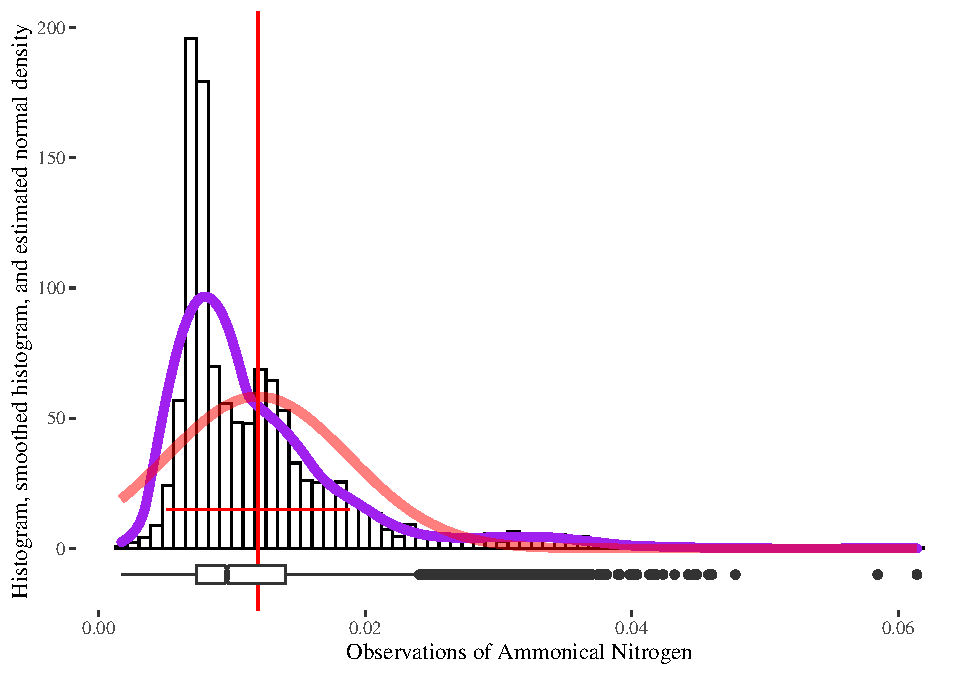
\includegraphics{Final-Report_files/figure-latex/nh4nhist-1.pdf}
\caption{\label{fig:nh4nhist}Histogram of Ammoniacal Nitrogen}
\end{figure}

Figure \ref{fig:chlahist} shows the distribution of Chlorophyll-A. We can see the fitted normal distribution differs slightly from the smoothed histogram. Table \ref{tab:laketable} shows the median is 3.9482 and the mean is 4.6093. The kurtosis is 18.3408, indicating the distribution of Chlorophyll-A is very heavy tailed, and the skewness is 2.5484, indicating the distribution is right skewed. A small proportion of the lakes exceeded the national bottomline of 12mg per cubic metre.

\begin{figure}
\centering
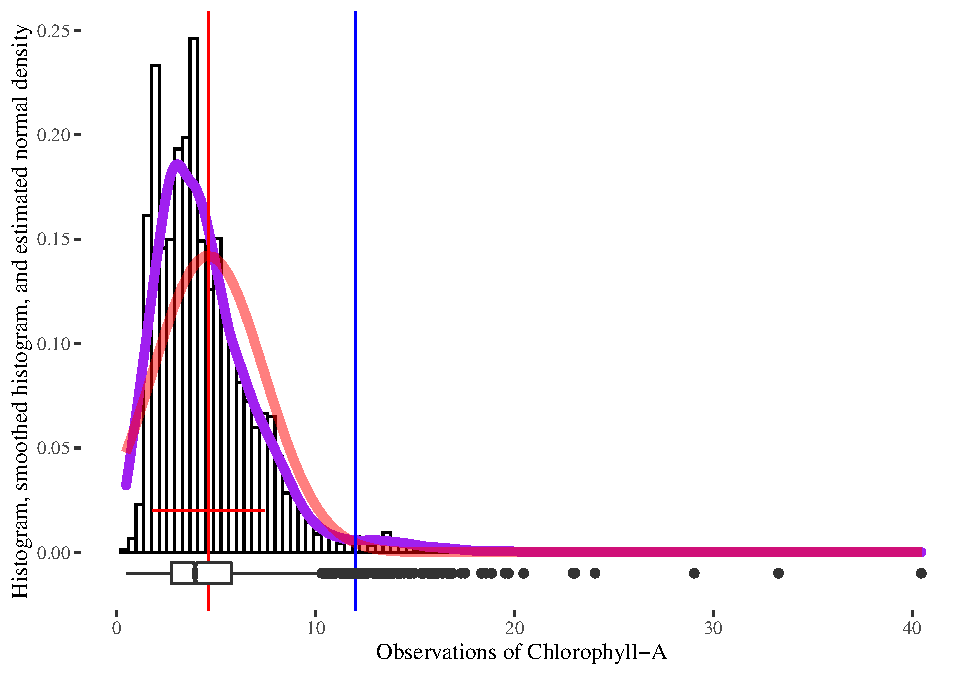
\includegraphics{Final-Report_files/figure-latex/chlahist-1.pdf}
\caption{\label{fig:chlahist}Histogram of Chlorophyll-A}
\end{figure}

Figure \ref{fig:tphist} shows the distribution of Total Phosphorus. The fitted normal distribution (red) fits quite well to the smoothed histogram (purple), although the kurtosis is very high, 26.2763. We would expect the kurtosis of a normally distributed variable to be close to 3 and with a skewness of 0, however the sample statistics of Total Phosphorus show the kurtosis much larger than 3 and the skewness 2.8722. This indicates the tails of this distribution are much heavier than a normal distribution, and it is right skewed. Table \ref{tab:laketable} shows the median of Total Phosphorus is 17.8966 mg per cubic meter, and the mean is 18.7206 mg per cubic meter. Few of the lakes exceeded the national bottomline of 50mg per cubic metre.

\begin{figure}
\centering
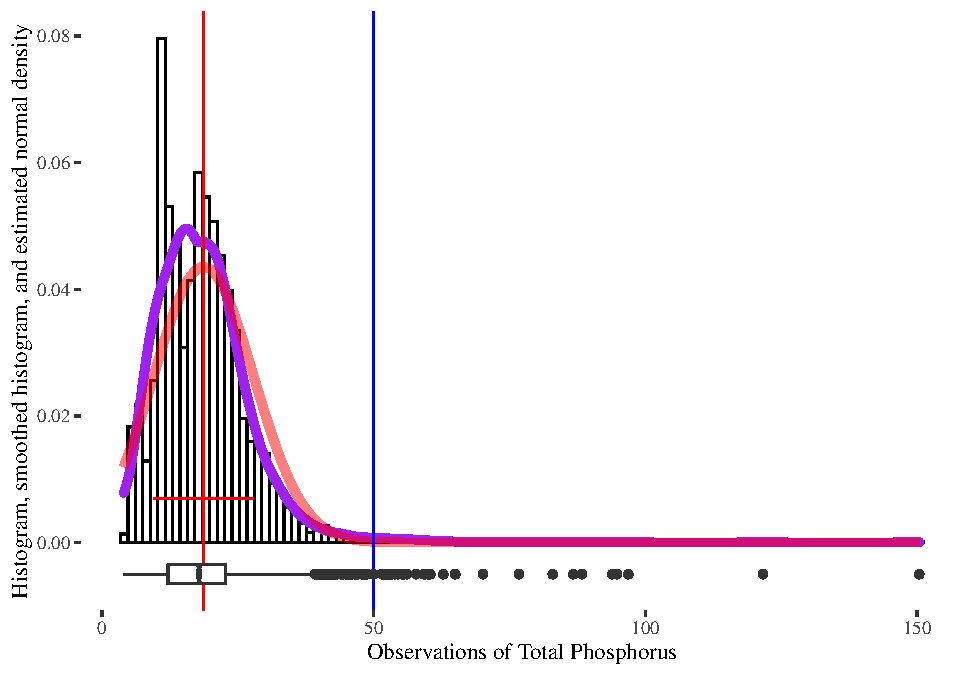
\includegraphics{Final-Report_files/figure-latex/tphist-1.pdf}
\caption{\label{fig:tphist}Histogram of Total Phosphorus}
\end{figure}

Figure \ref{fig:TNhist} shows the distribution of Total Nitrogen. The fitted normal distribution (in red) differs significantly from the smoothed histogram (purple). The smoothed histogram is more skewed and the mode is well below the mean. The median 416.7044 and mean 505.8606. Table \ref{tab:laketable} confirms this with a skewness of 1.0799. The kurtosis is 3.5463, indicating the distribution of Total Nitrogen has reasonable tails. A significant proportion of the observations exceed the higher of the two national bottomlines, of 800mg per cubic metre.

\begin{figure}
\centering
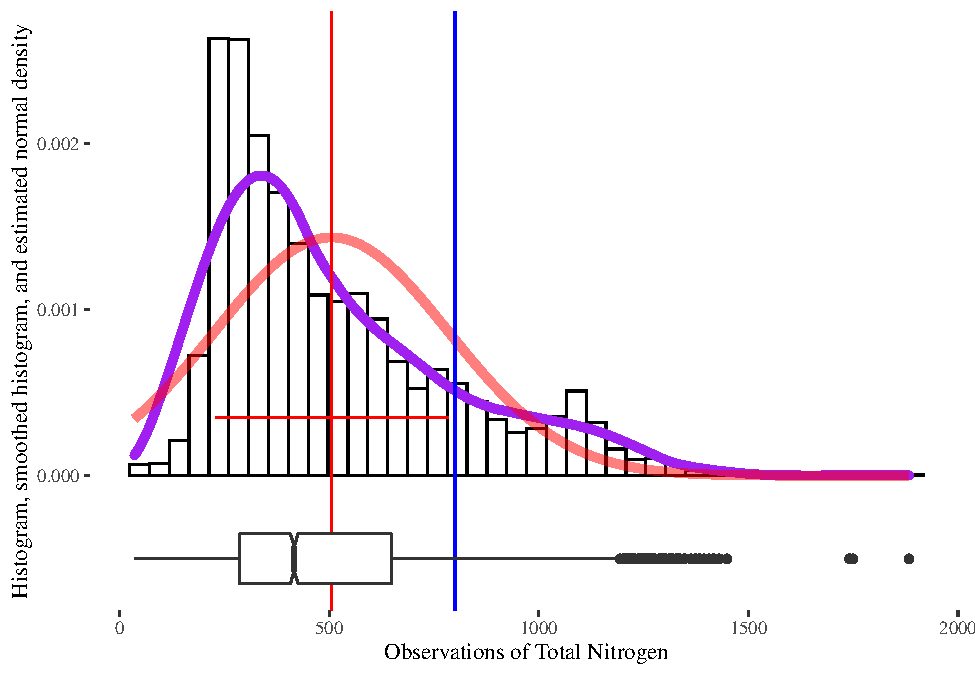
\includegraphics{Final-Report_files/figure-latex/TNhist-1.pdf}
\caption{\label{fig:TNhist}Histogram of Total Nitrogen}
\end{figure}

Figure \ref{fig:SECCHIhist} shows the distribution of Clarity. The fitted normal distribution (in red) differs from the smoothed histogram (purple). The smoothed histogram is slightly asymmetrical but not skewed, with a median of 4.4677 and a mean of 4.4510. Table \ref{tab:laketable} confirms this with a skewness of 0.2342. The kurtosis is 1.9983, indicating the distribution of Clarity has slightly lighter tails than a normal distribution. These statistics indicate the distribution of Clarity is close to normal.

\begin{figure}
\centering
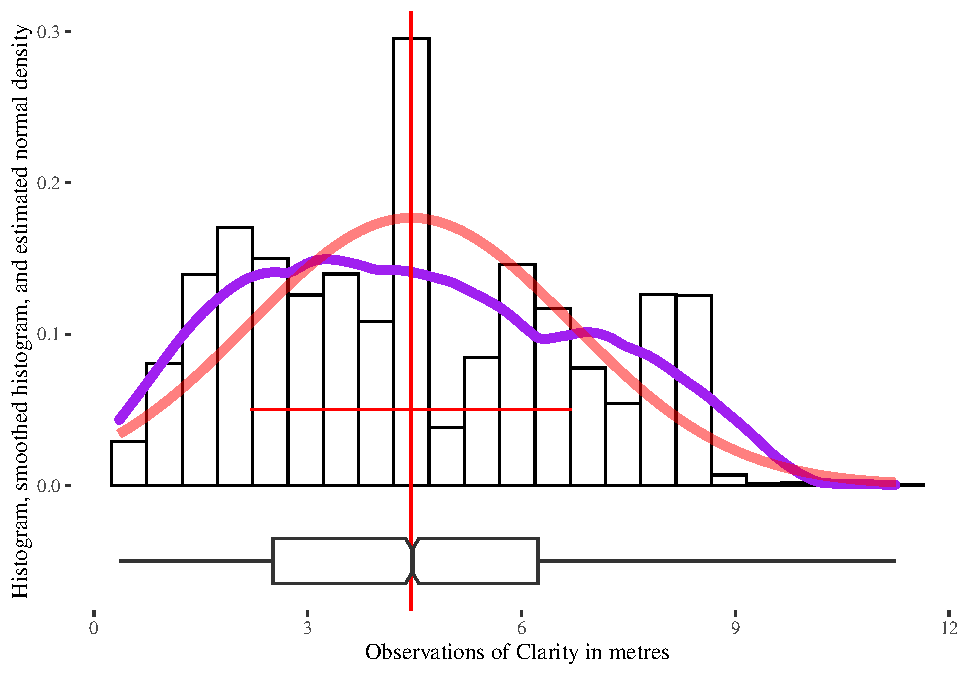
\includegraphics{Final-Report_files/figure-latex/SECCHIhist-1.pdf}
\caption{\label{fig:SECCHIhist}Histogram of Clarity (in metres)}
\end{figure}

We have made Cullen and Frey plots for Ammoniacal Nitrogen, Chlorophyll-A, Total Phosphorus, Total Nitrogen and Clarity, each with 1000 bootstrapped observations, shown in orange.

In figure \ref{fig:cfNH4N}, the Cullen and Frey graph of Ammoniacal Nitrogen, we can see the observed kurtosis and square of skewness was much larger than a normal distribution. The observation and all bootstrapped values were within the Beta distribution region, indicating the distribution of Ammoniacal Nitrogen in New Zealand lakes may follow a Beta distribution.

Figure \ref{fig:cfCHLA} shows the Cullen and Frey graph of Chlorophyll-A. The observed kurtosis and square of skewness were both much larger than we would expect for a normal distribution. The observed value and the bootstrapped observations lie on or just below the line all lognormal distributions lie on. This could tell us the distribution of Chlorophyll-A in New Zealand lakes could follow a lognormal distribution.

The Cullen and Frey graph of Total Phosphorus is shown in figure \ref{fig:cfTP}. The observed kurtosis and square of skewness were larger than both Ammoniacal Nitrogen and Chlorophyll-A. Similar to the Cullen and Frey graph of Chlorophyll-A, the observed value and bootstrapped observations seem to lie close to the line that contains all lognormal distributions. However, very few of the bootstrapped observations lie on this line, indicating Total Phosphorus in New Zealand lakes likely does not follow a lognormal, or any other distribution illustrated on this graph.

The Cullen and Frey graph of Total Nitrogen is shown in figure \ref{fig:cfTN}. The observed value and the boostrapped observations all lie within the grey area suggesting that Total Nitrogen follows a Beta distribution.

The Cullen and Frey graph of Clarity is shown in figure \ref{fig:cfSECCHI}. The observed value and bootstrapped values of the skewness and kurtosis of Clarity lies within the area all beta distributions exist within, and very close to the Uniform distributions, indicating the distribution of Clarity could be Uniform or Beta.

\begin{figure}
\centering
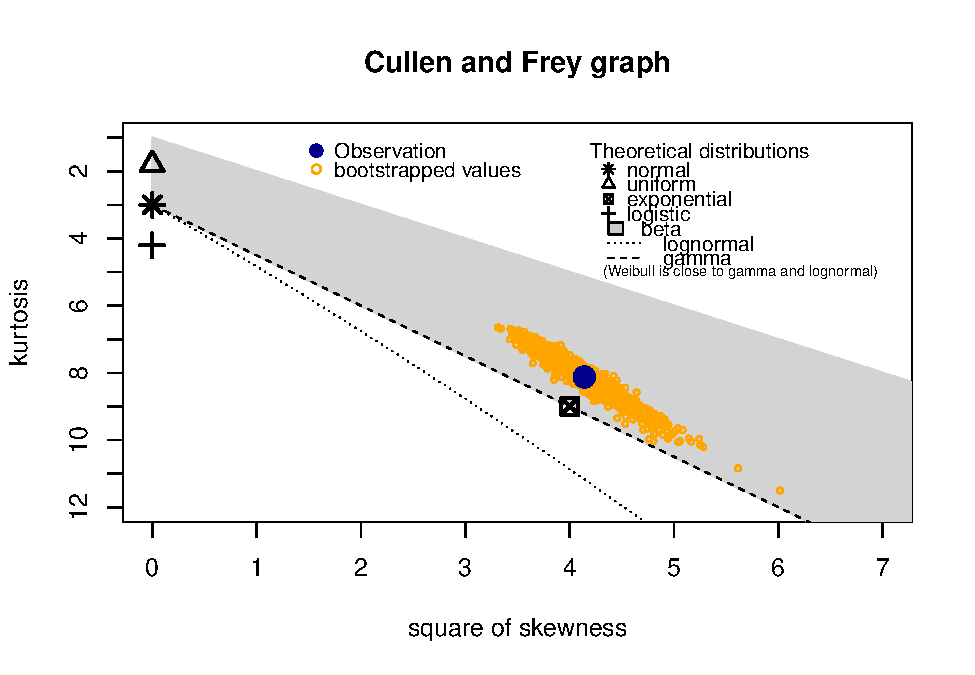
\includegraphics{Final-Report_files/figure-latex/cfNH4N-1.pdf}
\caption{\label{fig:cfNH4N}Cullen and Frey Graph of Ammoniacal Nitrogen}
\end{figure}

\begin{verbatim}
## summary statistics
## ------
## min:  0.001694   max:  0.061413 
## median:  0.009611 
## mean:  0.01195275 
## estimated sd:  0.006835817 
## estimated skewness:  2.034701 
## estimated kurtosis:  8.124069
\end{verbatim}

\begin{figure}
\centering
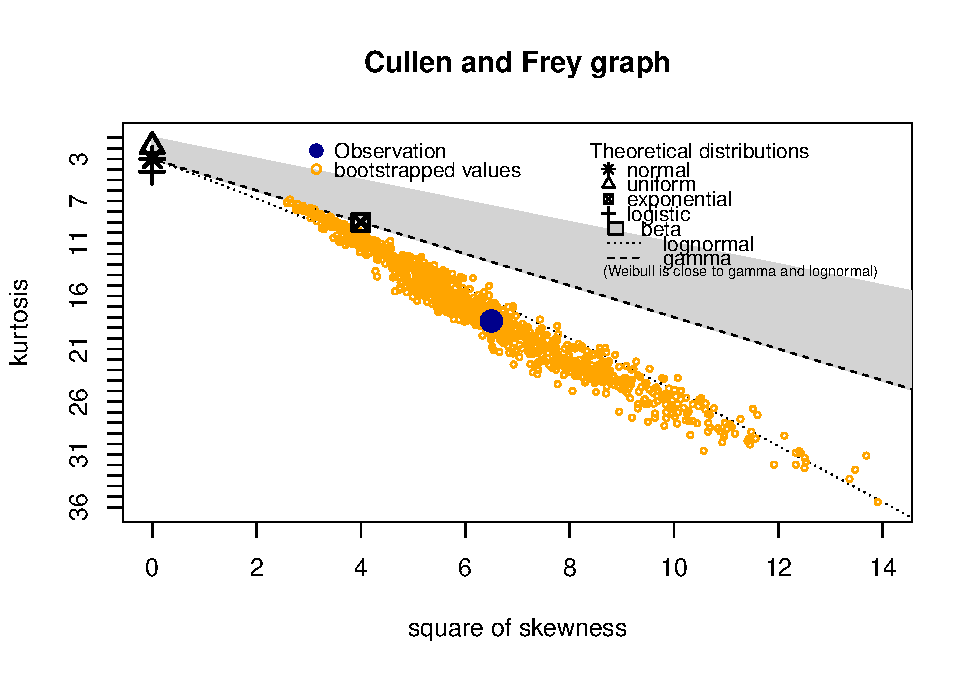
\includegraphics{Final-Report_files/figure-latex/cfCHLA-1.pdf}
\caption{\label{fig:cfCHLA}Cullen and Frey Graph of Chlorophyll-A}
\end{figure}

\begin{verbatim}
## summary statistics
## ------
## min:  0.473853   max:  40.44887 
## median:  3.948234 
## mean:  4.609289 
## estimated sd:  2.807067 
## estimated skewness:  2.549408 
## estimated kurtosis:  18.36258
\end{verbatim}

\begin{figure}
\centering
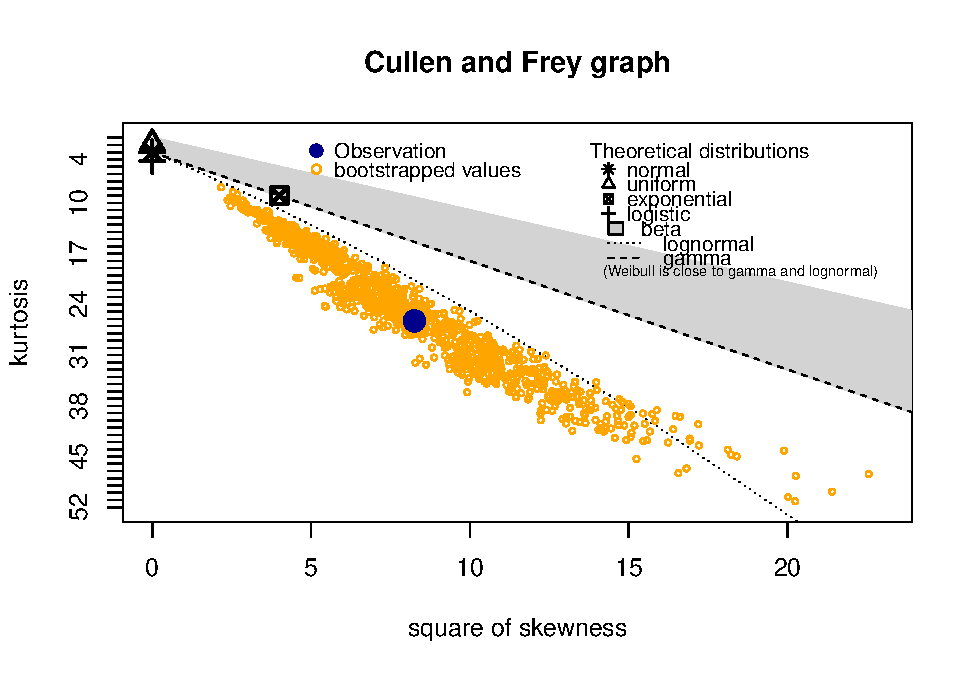
\includegraphics{Final-Report_files/figure-latex/cfTP-1.pdf}
\caption{\label{fig:cfTP}Cullen and Frey Graph of Total Phosphorus}
\end{figure}

\begin{verbatim}
## summary statistics
## ------
## min:  4.017657   max:  150.4168 
## median:  17.89664 
## mean:  18.72058 
## estimated sd:  9.143676 
## estimated skewness:  2.873323 
## estimated kurtosis:  26.27628
\end{verbatim}

\begin{figure}
\centering
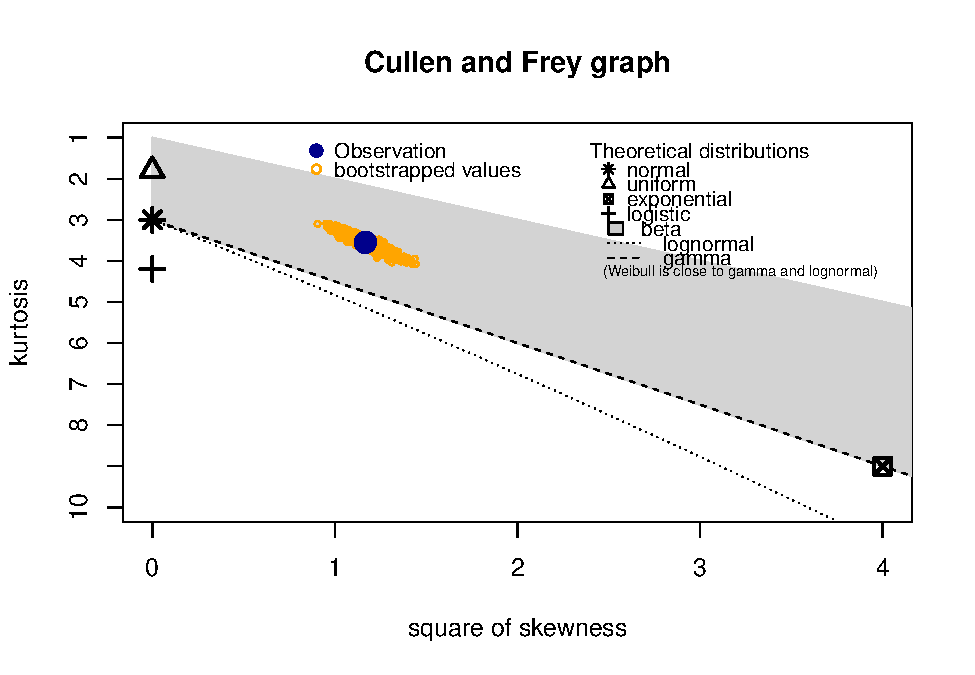
\includegraphics{Final-Report_files/figure-latex/cfTN-1.pdf}
\caption{\label{fig:cfTN}Cullen and Frey Graph of Total Nitrogen}
\end{figure}

\begin{verbatim}
## summary statistics
## ------
## min:  35.44473   max:  1883.172 
## median:  416.7044 
## mean:  505.8606 
## estimated sd:  277.9945 
## estimated skewness:  1.08037 
## estimated kurtosis:  3.548637
\end{verbatim}

\begin{figure}
\centering
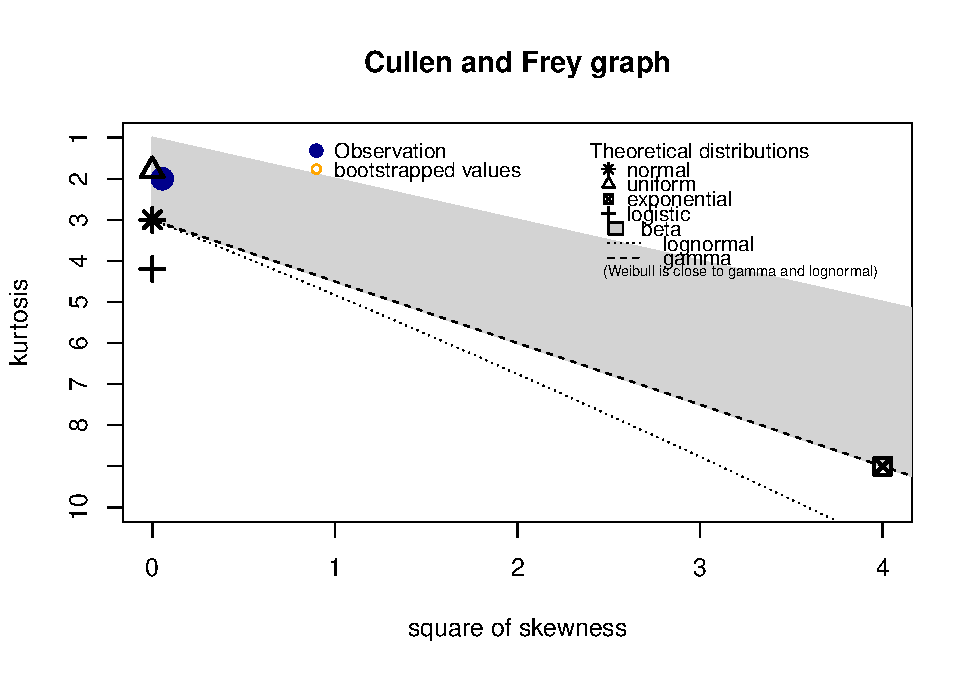
\includegraphics{Final-Report_files/figure-latex/cfSECCHI-1.pdf}
\caption{\label{fig:cfSECCHI}Cullen and Frey Graph of Clarity}
\end{figure}

\begin{verbatim}
## summary statistics
## ------
## min:  0.35536   max:  11.24885 
## median:  4.46773 
## mean:  4.450969 
## estimated sd:  2.255346 
## estimated skewness:  0.2342932 
## estimated kurtosis:  1.998537
\end{verbatim}

We believe, based on the Cullen and Frey graphs, none of these distributions are normal. We confirmed this with Anderson Darlings tests of normality. Table \ref{fig:adhealth} shows the test statistic and p-value for the Anderson Darling test on each Lake Health variable. The test statistics for Ammoniacal Nitrogen, Chlorophyll-A, Total Phosphorus, Total Nitrogen and Clarity are 226, 111, 68, 134 and 40, respectively (to the nearest whole number). For each variable, the p-value is 3e-24, confirming our suspicions that these variables are not normally distributed.

\begin{table}

\caption{\label{tab:adhealth}Anderson-Darling Test Statistic and P-value for the Lake Health Variables}
\centering
\begin{tabular}[t]{l|l|l|l|l|l}
\hline
  & Ammoniacal Nitrogen & Chlorophyll-A & Total Phosphorus & Total Nitrogen & Clarity\\
\hline
Test Statistic & 226.0701 & 111.2062 & 68.4039 & 133.6218 & 40.4676\\
\hline
P-Value & 3.7e-24 & 3.7e-24 & 3.7e-24 & 3.7e-24 & 3.7e-24\\
\hline
\end{tabular}
\end{table}

\hypertarget{univariate-analysis-of-the-lake-dimension-variables}{%
\paragraph{Univariate Analysis of the Lake Dimension Variables}\label{univariate-analysis-of-the-lake-dimension-variables}}

We produced histograms of each of the Lake Dimension Variables to examine their distributions.

\begin{figure}
\centering
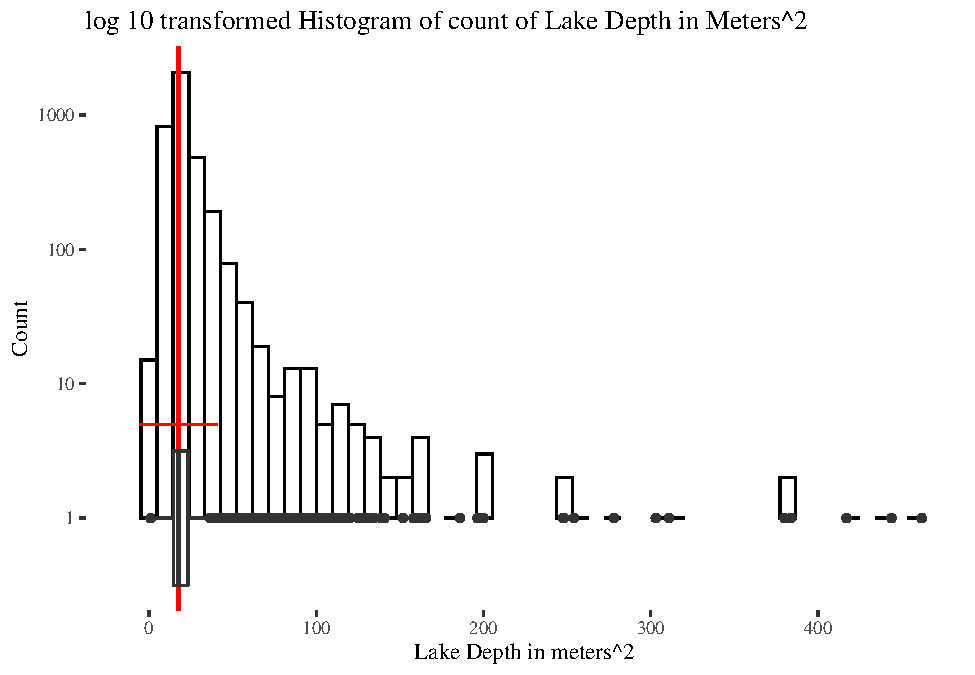
\includegraphics{Final-Report_files/figure-latex/HistDepth-1.pdf}
\caption{\label{fig:HistDepth}Log 10 transformed Histogram of Lake Depth in meters squared. Rectangles indicate skewed distribution, red vertical line indicates thge placement of the median value, red horizontal line indicates the placement of the median with one standard deviation.}
\end{figure}

Figure \ref{fig:HistDepth} shows the log 10 transformed histogram of the Lake Dimension Variable Lake Depth. We transformed it by log 10 to make the graph easier to interpret. The distribution of the graph is strongly skewed to the right, this is indicated by the boxplot at the bottom of the graph. Additionally from the boxplot we see that our data contains many outliers. The boxplot also suggests that with the removal of these outliers we may have a distribution that better approximates normal. We decided not to remove the outliers as these are still valid data points.

This distribution and interpretation of the above graph is very similar for all of the Lake Dimension variables; they all require log 10 transformation, they are all highly skewed, and appear to not approximate a normal distribution. As such we have not reproduced the histograms of the Lake Dimension variables Area and Perimeter here.

\hypertarget{multivariate-analysis-of-lake-health-variables}{%
\paragraph{Multivariate Analysis of Lake Health Variables}\label{multivariate-analysis-of-lake-health-variables}}

Table \ref{tab:corramat} shows the correlation matrix and figure \ref{fig:correlationplot} shows the visualization of this matrix. The strength of relationship is interpreted the size of the circles with strong relationships having larger circles and weaker relationships having small circles. Strength is also communicated via colour with darker colours indicating stronger relationship. Colour also indicates the direction of the relationship via a colour spectrum with reddish indicating a positive relationship, blue indicating a negative relationship and white indicating no relationship.

Ammoniacal Nitrogen has a weak, positive relationship with Chlorophyll-A (0.2076) and a Moderate, positive relationship with Total Phosphorus (0.3746). It has quite a strong relationship with Total Nitrogen (0.7294, which is to be expected asTotal Nitrogen includes Ammoniacal Nitrogen). Chlorophyll-A has a reasonably strong relationship with both Total Phosphorus (0.6939), and a moderate relationship with Total Nitrogen (0.5553). Total Phosphorus has a reasonable strong relationship with Total Nitrogen of (0.64533). These statistics suggest that there may be a positive relationship between the different molecules in water.

Clarity is the only variable to have any negative relationship with the other variables. Clarity has a negative correlation with all of the other variables of at least -0.5. It has an especially strong relationship with Total Nitrogen of -0.7823. These negative relationships are to be expected as it makes sense that an increase of other molecules in water would reduce the water's clarity. We can see this represented as dark blue circles in figure \ref{fig:correlationplot}.

\begin{table}

\caption{\label{tab:corramat}Correlation Matrix}
\centering
\begin{tabular}[t]{l|r|r|r|r|r}
\hline
  & Ammoniacal Nitrogen & Chlorophyll-A & Total Phosphorus & Total Nitrogen & Clarity\\
\hline
Ammoniacal Nitrogen & 1.0000000 & 0.2075794 & 0.3745765 & 0.7293838 & -0.5093412\\
\hline
Chlorophyll-A & 0.2075794 & 1.0000000 & 0.6938977 & 0.5552759 & -0.5847161\\
\hline
Total Phosphorus & 0.3745765 & 0.6938977 & 1.0000000 & 0.6453303 & -0.5336453\\
\hline
Total Nitrogen & 0.7293838 & 0.5552759 & 0.6453303 & 1.0000000 & -0.7823627\\
\hline
Clarity & -0.5093412 & -0.5847161 & -0.5336453 & -0.7823627 & 1.0000000\\
\hline
\end{tabular}
\end{table}

\begin{figure}
\centering
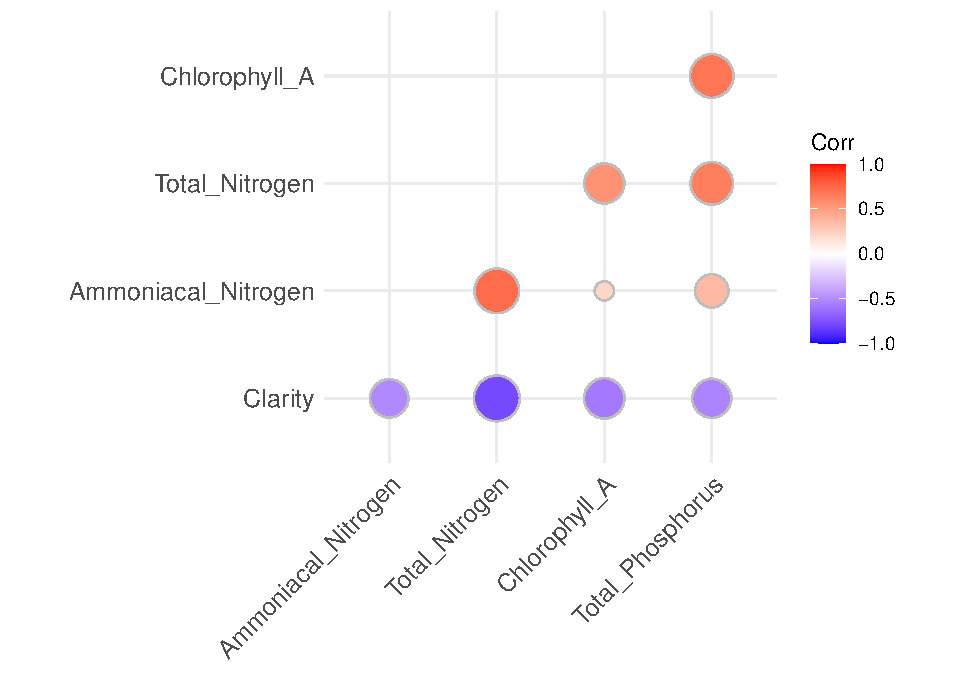
\includegraphics{Final-Report_files/figure-latex/correlationplot-1.pdf}
\caption{\label{fig:correlationplot}Visualisation of the Correlation Matrix}
\end{figure}

Figure \ref{fig:pairsplot} shows the pairs plot of the Lake Health variables, coloured by Dominant Landcover. We can see some separation between landcovers in the distribution of each variable. The relationships between Ammoniacal Nitrogen, Chlorophyll-A, Total Phosphorus and Total Nitrogen are positive, however all show non-constant scatter. It is also difficult to see any separation between the landcovers in these scatterplots as the data is dominated by Native and Pastoral landcovers (both have 1770 observations). The relationship between these four measures and Clarity are all negative, and appear to be non-linear. Another observation from this graph is that the correlations differ greatly between landcovers. For Ammoniacal Nitrogen and Chlorphyll-A, Native and Pastoral landcover groups have a weak positive correlation, while the other three types of landcover have weak negative correlations. The correlations between Ammoniacal Nitrogen and Total Phosphorus is similar for Exotic Forest, Native and Pastoral lakes (weak to moderate positive correlation), while the correlations for Other and Urban Area are very weak. For the rest of the pairs, the correlations for each landcover was similar, with either all positive or all negative correlations, ranging from 0.3 less to 0.3 more than the collective correlation. The two types of landcover that tended to differ most are the Other and Urban Area landcovers. This may be due to the small size of these groups (12 observations for Other and 85 observations for Urban Area).

\begin{figure}
\centering
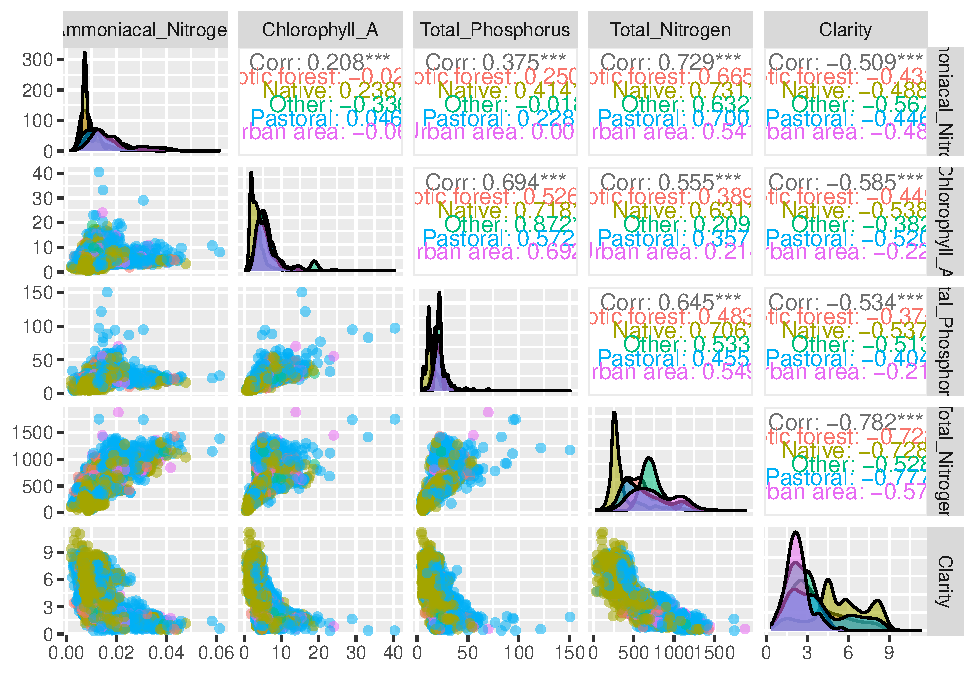
\includegraphics{Final-Report_files/figure-latex/pairsplot-1.pdf}
\caption{\label{fig:pairsplot}Pairs Plot of Lake Health}
\end{figure}

Next, we wanted to compare the distribution of the lake health variables by types of dominant landcover. Figure \ref{fig:boxNH4N} illustrates the box plots for each type of landcover. The observations have been log transformed to show the distributions better. We can see the highest 75\% of Ammoniacal Nitrogen measures in Urban areas are above the lower 75\% of measures in Exotic forest and Native landcovers. This could inidcate a relationship between landcover and Ammoniacal Nitrogen. Exotic forest and Native landcovers tend to have lower amounts of Ammoniacal Nitrogen in the lake water than in Pastoral, Urban and Other landcovers. The medians are shown in tables \ref{tab:eftabby}, \ref{tab:nattabby}, \ref{tab:ottabby}, \ref{tab:pasttabby} and \ref{tab:urbtabby} show the median Ammoniacal Nitrogen for lakes with Exotic forest, Native, Other, Pastoral and Urban dominant landcover to be 0.0084040, 0.0075540, 0.0123870, 0.0124780 and 0.0150880, respectively. There is a clear difference between the medians, with lower medians in Exotic forest and Native landcovers.

\begin{verbatim}
## notch went outside hinges. Try setting notch=FALSE.
\end{verbatim}

\begin{figure}
\centering
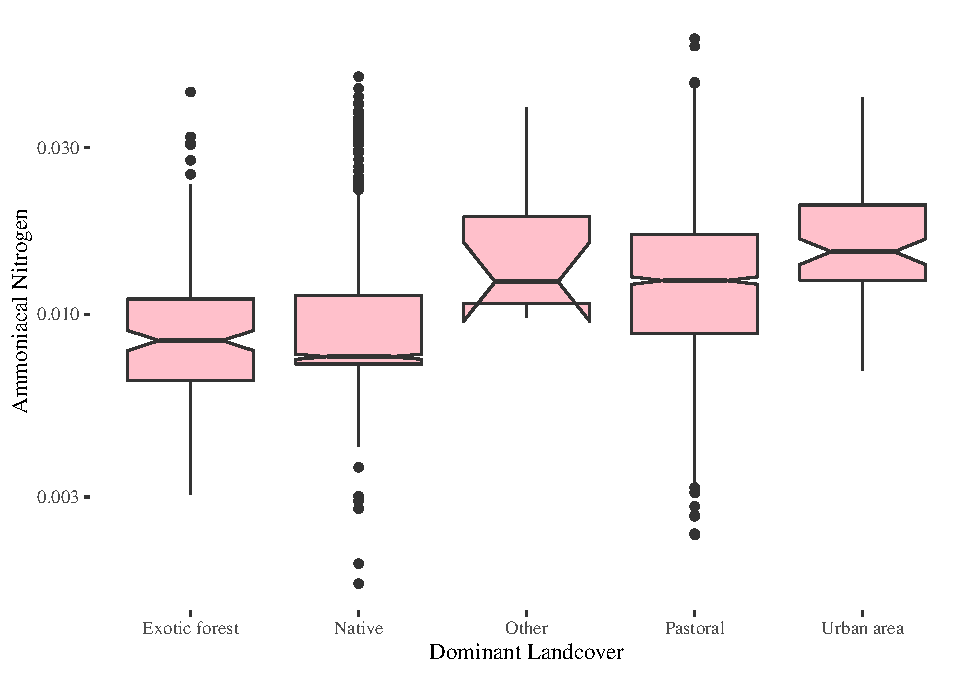
\includegraphics{Final-Report_files/figure-latex/boxNH4N-1.pdf}
\caption{\label{fig:boxNH4N}Box Plot of Landcover and Ammoniacal Nitrogen}
\end{figure}

Figure \ref{fig:boxCHLA} shows the distribution of Chlorophyll-A in each type of landcover. The observations have been log transformed to show the distributions better. We can see very similar distributions in Exotic forest, Other, Pastoral and Urban landcovers, however, lakes with Native landcover tended to have much lower levels of Chlorophyll-A than other landcovers. The medians support this, with the median Chlorophyll-A level of lakes with Native landcover being 2.8754, while all other types of landcover had medians above 5 mg per cubic meter (as shown in tables \ref{tab:eftabby}, \ref{tab:nattabby}, \ref{tab:ottabby}, \ref{tab:pasttabby} and \ref{tab:urbtabby}).

\begin{figure}
\centering
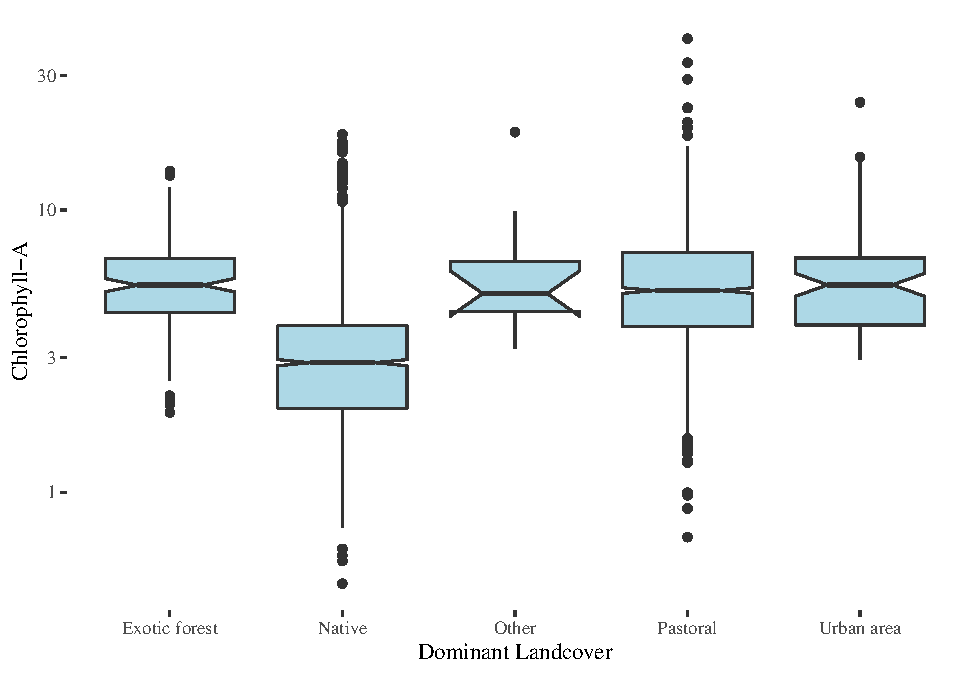
\includegraphics{Final-Report_files/figure-latex/boxCHLA-1.pdf}
\caption{\label{fig:boxCHLA}Box Plot of Landcover and Chlorophyll-A}
\end{figure}

Figure \ref{fig:boxTP} shows the distribution of Total Phosphorus for each type of dominant landcover. The observations have been log transformed to show the distributions better. The Native landcover group appears to have lower levels of Phosphorus than the other landcover types, with the third quantile being below the first quantile of all other categories.

Tables \ref{tab:eftabby}, \ref{tab:nattabby}, \ref{tab:ottabby}, \ref{tab:pasttabby} and \ref{tab:urbtabby} show the median levels of Phosphorus are 22.610470, 12.176880, 21.836995, 21.650210 and 21.416020 for Exotic forest, Native, Other, Pastoral and Urban landcovers, respectively. We can clearly see the level of Phosphorus in lakes with Native landcover tended to be much lower than other landcover types.

\begin{verbatim}
## notch went outside hinges. Try setting notch=FALSE.
\end{verbatim}

\begin{figure}
\centering
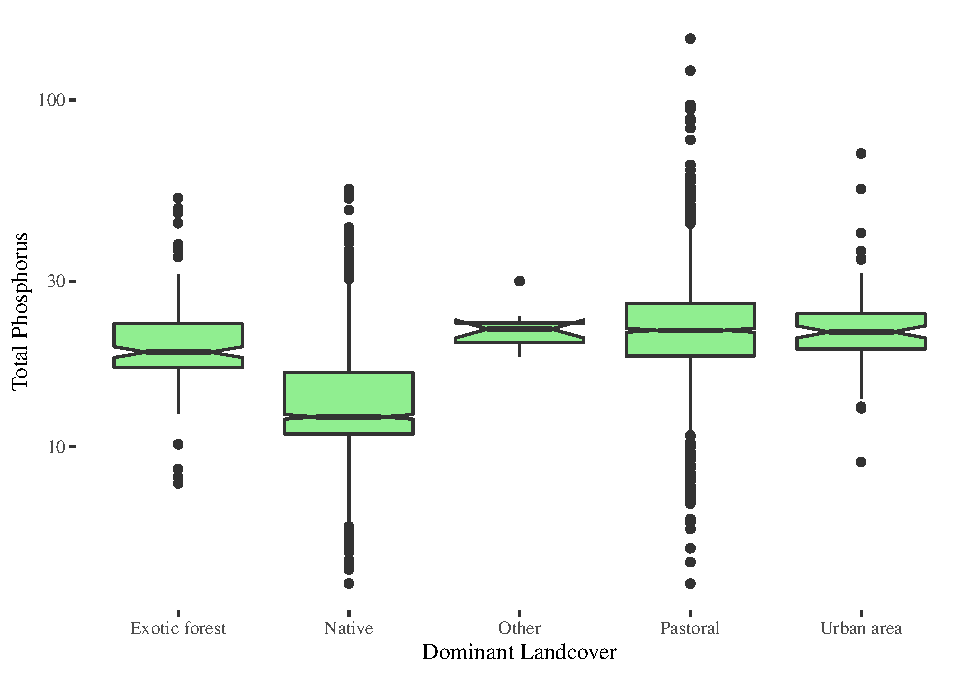
\includegraphics{Final-Report_files/figure-latex/boxTP-1.pdf}
\caption{\label{fig:boxTP}Box Plot of Landcover and Total Phosphorus}
\end{figure}

Figure \ref{fig:boxTN} shows the distributions of Total Nitrogen for each type of dominant landcover. Similarly to Ammoniacal Nitrogen, Chlorophyll-A and Total Phosphorus, the lakes with native landcover appeared to have lower levels of Total Nitrogen. The other types of dominant landcover appear to have very similar distributions, with the distribution of Total Nitrogen in lakes with Urban landcover being slightly higher. Tables \ref{tab:eftabby}, \ref{tab:nattabby}, \ref{tab:ottabby}, \ref{tab:pasttabby} and \ref{tab:urbtabby} show the median levels of Nitrogen are 556.8908, 286.4589, 724.3681, 558.8725 and 725.8646 for Exotic forest, Native, Other, Pastoral and Urban landcovers, respectively. These statistics support the claim that lakes with Native landcover tend to have lower levels of Nitrogen than other types of dominant landcover.

\begin{verbatim}
## notch went outside hinges. Try setting notch=FALSE.
\end{verbatim}

\begin{figure}
\centering
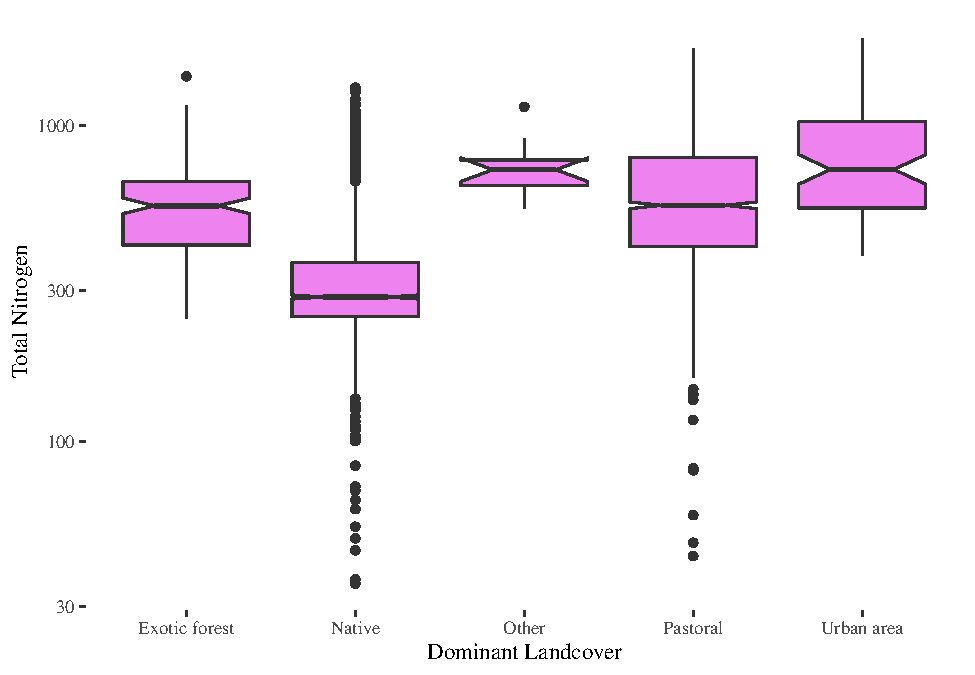
\includegraphics{Final-Report_files/figure-latex/boxTN-1.pdf}
\caption{\label{fig:boxTN}Box Plot of Landcover and Total Nitrogen}
\end{figure}

The distribution of Clarity by dominant landcover is shown in figure \ref{fig:boxSECCHI}. The lakes with Native landcover appear to have a higher clarity, or appear clearer than lakes with other types of dominant landcover. Lakes with Urban or `Other' landcover are less clear. This is to be expected as we have found that higher levels of Ammoniacal Nitrogen, Chlorophyll-A, Total Phosphorus and Total Nitrogen are associated with lower levels of Clarity. Tables \ref{tab:eftabby}, \ref{tab:nattabby}, \ref{tab:ottabby}, \ref{tab:pasttabby} and \ref{tab:urbtabby} show the median levels of Clarity are 2.9450, 5.4663, 2.3282, 3.3240 and 2.1811 for Exotic forest, Native, Other, Pastoral and Urban landcovers, respectively. We can say that lakes with Native landcover tend to be clearer than lakes with other types of dominant landcover.

\begin{verbatim}
## notch went outside hinges. Try setting notch=FALSE.
\end{verbatim}

\begin{figure}
\centering
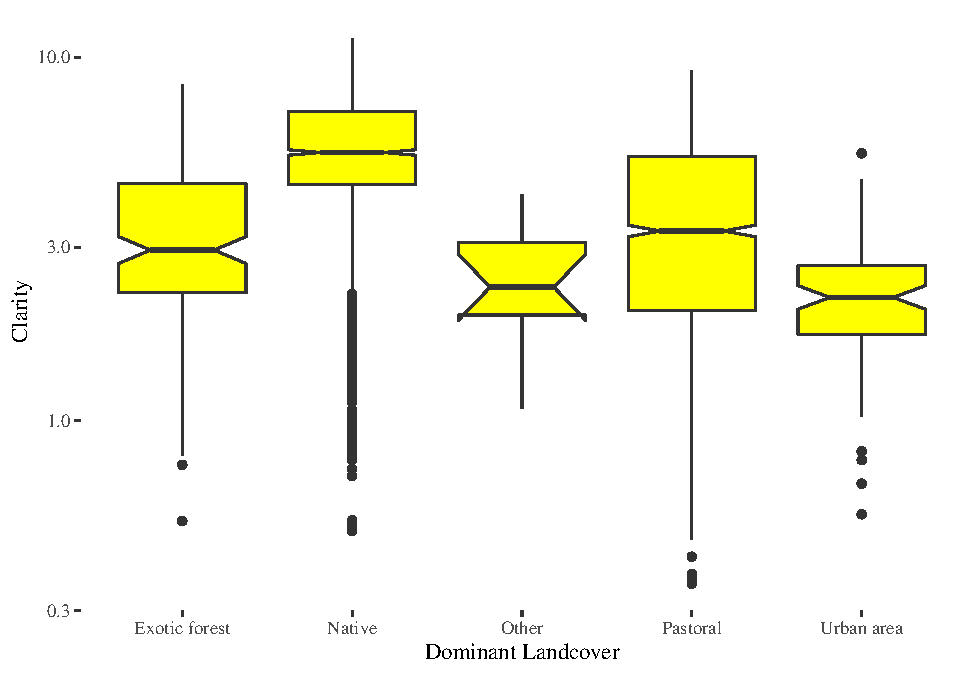
\includegraphics{Final-Report_files/figure-latex/boxSECCHI-1.pdf}
\caption{\label{fig:boxSECCHI}Box Plot of Landcover and Clarity}
\end{figure}

\begin{longtable}[]{@{}lrrrrr@{}}
\caption{\label{tab:eftabby}Table of Sample Statistics for Exotic Forest Landcover}\tabularnewline
\toprule()
& Ammoniacal Nitrogen & Chlorophyll-A & Total Phosphorus & Total Nitrogen & Clarity \\
\midrule()
\endfirsthead
\toprule()
& Ammoniacal Nitrogen & Chlorophyll-A & Total Phosphorus & Total Nitrogen & Clarity \\
\midrule()
\endhead
Sample Size & 165.0000000 & 165.000000 & 165.000000 & 165.000000 & 165.0000000 \\
Minimum & 0.0030560 & 1.914920 & 7.824604 & 244.552300 & 0.5283680 \\
1st Quantile & 0.0064500 & 4.327840 & 16.903240 & 418.269100 & 2.2472620 \\
Median & 0.0084040 & 5.411983 & 18.720890 & 556.890800 & 2.9450360 \\
3rd Quantile & 0.0110560 & 6.729298 & 22.610470 & 663.692100 & 4.4890560 \\
Maximum & 0.0432230 & 13.748320 & 52.192960 & 1430.616000 & 8.3944250 \\
Standard Deviation & 0.0059558 & 2.251981 & 7.172119 & 205.723829 & 1.8382921 \\
Mean & 0.0101148 & 5.759535 & 20.640032 & 577.841100 & 3.4546657 \\
Kurtosis & 10.9583216 & 5.440503 & 8.390341 & 4.213177 & 3.0542778 \\
Skewness & 2.5252855 & 1.306315 & 2.056528 & 1.066055 & 0.8963324 \\
\bottomrule()
\end{longtable}

\begin{longtable}[]{@{}lrrrrr@{}}
\caption{\label{tab:nattabby}Table of Sample Statistics for Native Landcover}\tabularnewline
\toprule()
& Ammoniacal Nitrogen & Chlorophyll-A & Total Phosphorus & Total Nitrogen & Clarity \\
\midrule()
\endfirsthead
\toprule()
& Ammoniacal Nitrogen & Chlorophyll-A & Total Phosphorus & Total Nitrogen & Clarity \\
\midrule()
\endhead
Sample Size & 1770.0000000 & 1770.000000 & 1770.000000 & 1770.000000 & 1770.0000000 \\
Minimum & 0.0016940 & 0.473853 & 4.020834 & 35.444730 & 0.4966520 \\
1st Quantile & 0.0072020 & 1.984959 & 10.870083 & 248.086550 & 4.4677300 \\
Median & 0.0075540 & 2.875430 & 12.176880 & 286.458900 & 5.4663295 \\
3rd Quantile & 0.0113143 & 3.884066 & 16.351820 & 367.934700 & 7.0846440 \\
Maximum & 0.0477830 & 18.554890 & 55.290970 & 1317.353000 & 11.2488500 \\
Standard Deviation & 0.0053919 & 2.024765 & 6.085992 & 203.570216 & 2.0869312 \\
Mean & 0.0098571 & 3.310055 & 13.856583 & 360.579423 & 5.3440779 \\
Kurtosis & 14.5213007 & 15.904375 & 8.898851 & 6.930813 & 2.4458642 \\
Skewness & 3.1201691 & 2.918515 & 1.826233 & 2.035596 & -0.2370482 \\
\bottomrule()
\end{longtable}

\begin{longtable}[]{@{}lrrrrr@{}}
\caption{\label{tab:ottabby}Table of Sample Statistics for Other Landcover}\tabularnewline
\toprule()
& Ammoniacal Nitrogen & Chlorophyll-A & Total Phosphorus & Total Nitrogen & Clarity \\
\midrule()
\endfirsthead
\toprule()
& Ammoniacal Nitrogen & Chlorophyll-A & Total Phosphorus & Total Nitrogen & Clarity \\
\midrule()
\endhead
Sample Size & 12.0000000 & 12.000000 & 12.000000 & 12.000000 & 12.0000000 \\
Minimum & 0.0097610 & 3.235230 & 18.167920 & 545.199500 & 1.0783810 \\
1st Quantile & 0.0107397 & 4.381197 & 19.930630 & 644.760175 & 1.9537652 \\
Median & 0.0123870 & 5.055644 & 21.836995 & 724.368100 & 2.3281925 \\
3rd Quantile & 0.0190660 & 6.590519 & 22.724430 & 778.679350 & 3.0892158 \\
Maximum & 0.0389650 & 18.851460 & 30.023000 & 1144.875000 & 4.1946350 \\
Standard Deviation & 0.0085389 & 4.319832 & 3.147497 & 158.740455 & 0.9114810 \\
Mean & 0.0160571 & 6.517253 & 21.893479 & 745.837125 & 2.4852789 \\
Kurtosis & 5.3078064 & 6.712099 & 4.854776 & 4.404853 & 2.2352235 \\
Skewness & 1.7485667 & 2.135868 & 1.300069 & 1.324778 & 0.2319556 \\
\bottomrule()
\end{longtable}

\begin{longtable}[]{@{}lrrrrr@{}}
\caption{\label{tab:pasttabby}Table of Sample Statistics for Pastoral Landcover}\tabularnewline
\toprule()
& Ammoniacal Nitrogen & Chlorophyll-A & Total Phosphorus & Total Nitrogen & Clarity \\
\midrule()
\endfirsthead
\toprule()
& Ammoniacal Nitrogen & Chlorophyll-A & Total Phosphorus & Total Nitrogen & Clarity \\
\midrule()
\endhead
Sample Size & 1770.0000000 & 1770.000000 & 1770.000000 & 1770.0000000 & 1770.0000000 \\
Minimum & 0.0023340 & 0.692440 & 4.017657 & 43.3438700 & 0.3553600 \\
1st Quantile & 0.0088040 & 3.856655 & 18.244765 & 413.5380500 & 2.0109795 \\
Median & 0.0124780 & 5.180067 & 21.650210 & 558.8725000 & 3.3239965 \\
3rd Quantile & 0.0169287 & 7.067774 & 25.933367 & 792.1972000 & 5.3363585 \\
Maximum & 0.0614130 & 40.448870 & 150.416800 & 1749.8950000 & 9.2128900 \\
Standard Deviation & 0.0073402 & 2.920128 & 9.464692 & 275.1740646 & 2.1464743 \\
Mean & 0.0139015 & 5.715493 & 23.177153 & 629.6969317 & 3.7689957 \\
Kurtosis & 6.6581435 & 23.631222 & 37.838715 & 2.9395897 & 2.3785691 \\
Skewness & 1.5961889 & 2.942548 & 4.067867 & 0.7974652 & 0.6671145 \\
\bottomrule()
\end{longtable}

\begin{longtable}[]{@{}lrrrrr@{}}
\caption{\label{tab:urbtabby}Table of Sample Statistics for Urban Landcover}\tabularnewline
\toprule()
& Ammoniacal Nitrogen & Chlorophyll-A & Total Phosphorus & Total Nitrogen & Clarity \\
\midrule()
\endfirsthead
\toprule()
& Ammoniacal Nitrogen & Chlorophyll-A & Total Phosphorus & Total Nitrogen & Clarity \\
\midrule()
\endhead
Sample Size & 85.0000000 & 85.000000 & 85.000000 & 85.0000000 & 85.0000000 \\
Minimum & 0.0068880 & 2.942836 & 9.029183 & 387.4383000 & 0.5520370 \\
1st Quantile & 0.0125150 & 3.912775 & 19.107640 & 548.3017000 & 1.7239980 \\
Median & 0.0150880 & 5.427137 & 21.416020 & 725.8646000 & 2.1811430 \\
3rd Quantile & 0.0205250 & 6.755165 & 24.147820 & 1027.0020000 & 2.6690640 \\
Maximum & 0.0417070 & 24.052490 & 70.108590 & 1883.1720000 & 5.4404300 \\
Standard Deviation & 0.0083745 & 3.389789 & 8.392760 & 286.3296449 & 0.8785109 \\
Mean & 0.0180000 & 6.126680 & 23.030843 & 778.8134400 & 2.2658755 \\
Kurtosis & 3.4495705 & 11.658444 & 15.327134 & 4.1074614 & 4.5139920 \\
Skewness & 1.1230235 & 2.512231 & 2.892799 & 0.9219365 & 0.8943855 \\
\bottomrule()
\end{longtable}

We wanted to run tests for a difference in mean of each Lake Health variable for each type of landcover, but we first needed to check the normality assumptions to ascertain which tests we could conduct. If any one of these groups does not meet the normality assumption, normality cannot be assumed for these tests. To test this we conducted Anderson-Darling tests on just the Native landcover group.

Table \ref{fig:adhelth} shows the test statistic and p-value for the Anderson Darling test on each Lake Health variable for the Native landcover. The test statistics for Ammoniacal Nitrogen, Chlorophyll-A, Total Phosphorus, Total Nitrogen and Clarity are 209, 92, 58, 168 and 21, respectively (to the nearest whole number). For each variable, the p-value is 3e-24, confirming our suspicions that the distribution of the Lake Health variables for Native lakes are not normally distributed, violating the normality assumption. We conducted this test on every type of landcover with similar results.

\begin{table}

\caption{\label{tab:adhelth}Anderson-Darling Test Statistic and P-value for the Lake Health Variables by Native Landcover}
\centering
\begin{tabular}[t]{l|l|l|l|l|l}
\hline
  & Ammoniacal Nitrogen & Chlorophyll-A & Total Phosphorus & Total Nitrogen & Clarity\\
\hline
Test Statistic & 208.5689 & 91.6093 & 58.2436 & 167.8357 & 21.0911\\
\hline
P-Value & 3.7e-24 & 3.7e-24 & 3.7e-24 & 3.7e-24 & 3.7e-24\\
\hline
\end{tabular}
\end{table}

We analysed the relationship between the Lake Health variables and Region.

\begin{table}

\caption{\label{tab:sec}Regional Mean and Median Lake Health}
\centering
\resizebox{\linewidth}{!}{
\begin{tabular}[t]{l|r|r|l|r|r|l|r|r|l|r|r|l|r|r}
\hline
Region & Mean\_NH4N & Median\_NH4N & Region & Mean\_CHLA & Median\_CHLA & Region & Mean\_TP & Median\_TP & Region & Mean\_TN & Median\_TN & Region & Mean\_SECCHI & Median\_SECCHI\\
\hline
Waikato & 0.0169931 & 0.0123660 & Gisborne & 7.808367 & 7.351853 & Taranaki & 24.60256 & 24.83678 & Waikato & 790.2603 & 791.5458 & Wellington & 2.182703 & 1.734104\\
\hline
Wellington & 0.0166320 & 0.0134980 & Taranaki & 7.176843 & 7.110607 & Gisborne & 26.26159 & 23.86373 & Wellington & 708.1088 & 722.2273 & Waikato & 3.108126 & 2.461897\\
\hline
Gisborne & 0.0160306 & 0.0132765 & Hawke's Bay & 6.809741 & 6.649401 & Waikato & 23.23461 & 22.29681 & Gisborne & 700.7699 & 680.4638 & Auckland & 2.635606 & 2.596739\\
\hline
Manawatū-Whanganui & 0.0143978 & 0.0110985 & Waikato & 7.115944 & 6.156554 & Manawatū-Whanganui & 24.04704 & 21.75352 & Taranaki & 574.7697 & 563.5217 & Gisborne & 3.033813 & 2.757868\\
\hline
Marlborough district council & 0.0138354 & 0.0097970 & Northland & 5.503763 & 5.421323 & Hawke's Bay & 21.36501 & 21.60229 & Manawatū-Whanganui & 709.0396 & 555.2100 & Northland & 3.121884 & 2.803300\\
\hline
Auckland & 0.0134935 & 0.0115450 & Wellington & 6.890644 & 5.391158 & Wellington & 23.06120 & 21.30178 & Northland & 553.4311 & 550.2800 & Taranaki & 3.216804 & 3.109920\\
\hline
Canterbury & 0.0133163 & 0.0131270 & Manawatū-Whanganui & 5.896478 & 5.356666 & Marlborough district council & 19.68485 & 19.60149 & Hawke's Bay & 558.7630 & 535.7862 & Manawatū-Whanganui & 3.582909 & 3.119695\\
\hline
Bay of Plenty & 0.0128409 & 0.0098540 & Auckland & 5.925387 & 5.335608 & Bay of Plenty & 20.54074 & 19.54886 & Marlborough district council & 522.9138 & 527.1625 & Hawke's Bay & 3.606981 & 3.416575\\
\hline
Otago & 0.0127451 & 0.0120175 & Bay of Plenty & 5.670382 & 4.981374 & Otago & 20.69889 & 19.01017 & Auckland & 534.9663 & 486.0566 & Marlborough district council & 4.336709 & 4.020992\\
\hline
Hawke's Bay & 0.0114907 & 0.0096720 & West Coast & 4.128556 & 3.522108 & Canterbury & 20.03111 & 17.96068 & Bay of Plenty & 573.8112 & 451.1150 & Bay of Plenty & 4.182245 & 4.183662\\
\hline
West Coast & 0.0111620 & 0.0087230 & Marlborough district council & 4.418469 & 3.506617 & Northland & 18.36308 & 17.88858 & Canterbury & 481.9375 & 379.6930 & West Coast & 4.680724 & 4.601896\\
\hline
Taranaki & 0.0101370 & 0.0101145 & Canterbury & 3.523742 & 3.334410 & Auckland & 19.11667 & 17.33723 & Otago & 422.0329 & 367.6522 & Southland & 5.138127 & 4.616884\\
\hline
Southland & 0.0099627 & 0.0074620 & Otago & 3.326594 & 3.219797 & Tasman district council & 17.77295 & 15.33291 & West Coast & 492.6764 & 365.7440 & Tasman district council & 4.691611 & 5.709074\\
\hline
Tasman district council & 0.0091943 & 0.0072210 & Southland & 3.258189 & 3.073008 & West Coast & 16.99558 & 15.10845 & Southland & 373.3848 & 295.8158 & Otago & 5.395194 & 5.727244\\
\hline
Northland & 0.0089272 & 0.0075225 & Tasman district council & 5.150028 & 2.920793 & Southland & 13.71377 & 11.43682 & Tasman district council & 448.2798 & 295.3265 & Canterbury & 5.546141 & 5.743230\\
\hline
\end{tabular}}
\end{table}

\hypertarget{multivariate-analysis-of-the-lake-dimension-variables}{%
\paragraph{Multivariate analysis of the Lake Dimension variables}\label{multivariate-analysis-of-the-lake-dimension-variables}}

\hypertarget{examining-the-correlation-between-area-depth-and-perimeter-need-to-edit-referencing-and-titles}{%
\paragraph{Examining the Correlation between Area, Depth and Perimeter NEED TO EDIT REFERENCING AND TITLES}\label{examining-the-correlation-between-area-depth-and-perimeter-need-to-edit-referencing-and-titles}}

*Correlation matrix rounded to three decimal place

\begin{verbatim}
##                lake_perimeter lake_depth lake_area
## lake_perimeter          1.000      0.780     0.797
## lake_depth              0.780      1.000     0.518
## lake_area               0.797      0.518     1.000
\end{verbatim}

Visualisation of the Correlation Matrix:

\begin{figure}
\centering
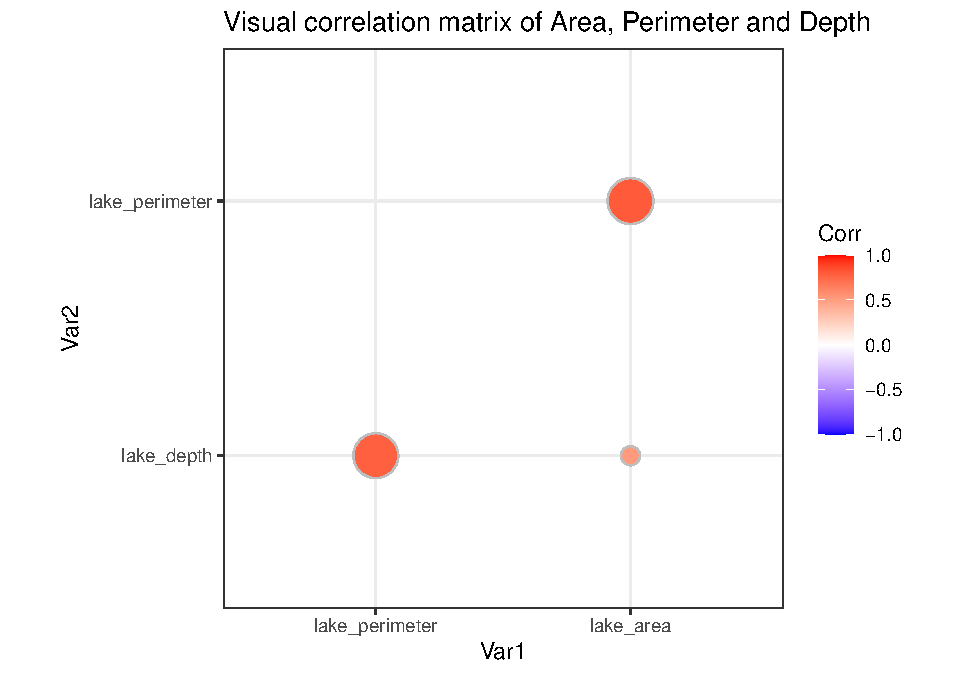
\includegraphics{Final-Report_files/figure-latex/VisCorr1-1.pdf}
\caption{\label{fig:VisCorr1}Visual of the correlation between, depth, perimeter and area where Strength and direction of relationship are indicated by circle size and colour}
\end{figure}

As to be expected, the three Lake Dimension have positive correlations with one another. The correlation between lake area and lake depth isn't small but it is smaller than one may expect. Lake Perimeter has a rather strong relationship with both area and depth.

\hypertarget{results}{%
\subsection{Results}\label{results}}

\begin{itemize}
\tightlist
\item
  test for difference in means health/land + pairwise tests
\item
  PCA
\item
  FA
\end{itemize}

\hypertarget{linear-discriminant-analysis-and-factor-analysis}{%
\subsubsection{Linear Discriminant Analysis and Factor Analysis}\label{linear-discriminant-analysis-and-factor-analysis}}

After finishing our Preliminary Report we also looked at ways we could implement Factor Analysis (FA) and Linear Discriminant Analysis (LDA) with our data.

\hypertarget{linear-discriminant-analysis}{%
\paragraph{Linear Discriminant Analysis}\label{linear-discriminant-analysis}}

For LDA, we wanted to see if there was potential to implement LDA if there was information loss. As such, we attempted to predict which Dominant Landcover a lake was, based on the Lake Health Variables.

Reminder - the categories that dominant landcover can take on are: Pastoral, Native, Urban area, Exotic forest, and Other

We first scaled the Lake Health Variables. We then randomly created training and test sets with 70\% of the data in the training set and 30\% in the test set. We then fit the LDA model using the train data. The output was shown below.

\begin{verbatim}
## Call:
## lda(dominant_landcover ~ ., data = train)
## 
## Prior probabilities of groups:
## Exotic forest        Native         Other      Pastoral    Urban area 
##   0.045505829   0.461827755   0.003384731   0.464836405   0.024445280 
## 
## Group means:
##               median_TN_mg.m.3 median_CHLA_mg.m.3 median_SECCHI_metre
## Exotic forest        0.2730316          0.4435337          -0.4154415
## Native              -0.5062055         -0.4594529           0.3971934
## Other                1.0258008          0.6837159          -0.9124731
## Pastoral             0.4459826          0.4091680          -0.3274973
## Urban area           1.0525270          0.6213234          -0.9667699
##               median_TP_mg.m.3 median_NH4N_mg.L..1
## Exotic forest        0.2275124          -0.2646927
## Native              -0.5223730          -0.2933420
## Other                0.3777788           0.7550298
## Pastoral             0.4988880           0.2623736
## Urban area           0.5386756           0.8953922
## 
## Coefficients of linear discriminants:
##                            LD1        LD2        LD3         LD4
## median_TN_mg.m.3    -0.8323879 -0.7181879  0.1465040  1.21592998
## median_CHLA_mg.m.3  -0.3431264 -0.1201895  0.1163328  1.01510707
## median_SECCHI_metre -0.2016573  0.5174212 -0.6676406  1.41899817
## median_TP_mg.m.3    -0.4412428  0.4565318 -1.0312835 -0.95252709
## median_NH4N_mg.L..1  0.1122687  1.3228239  0.4631494 -0.06801566
## 
## Proportion of trace:
##    LD1    LD2    LD3    LD4 
## 0.9166 0.0483 0.0347 0.0004
\end{verbatim}

From the Prior Probabilities we see that Pastoral Landcover and Native Landcover each explain about 46\% of the prior probabilities in the training set.

From examining the coefficients of the linear discriminants, it seems that Total nitrogen (TN) impacts the first linear discriminant the most (-0.8323.).

Examining the proportion of traces we see that the LD1 accounts for approximately 91 percent of the separation. LD2 and LD3 account for approximately 4.8 and 3.5 percent of the separation respectively. The remainder is explained by LD4.

We produced a partition plot to examine the separation.

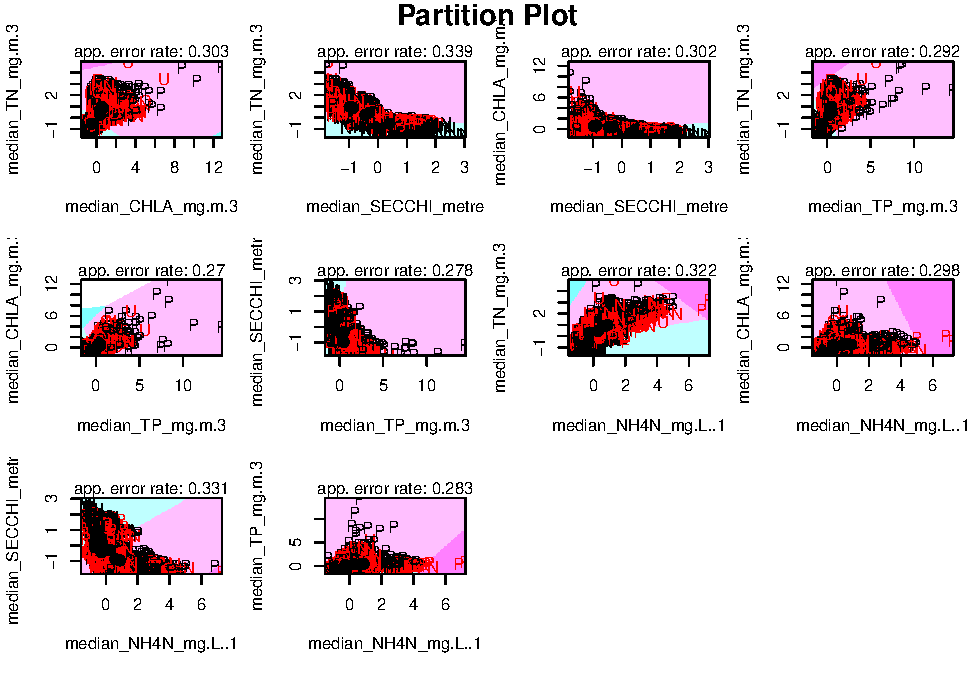
\includegraphics{Final-Report_files/figure-latex/unnamed-chunk-3-1.pdf}

It is difficult to get much useful information from the the Partition Plot. What we can see is that there is a reasonable number of errors. We can also see is that most of the data seems to be in two of the partitions and some of the partitions have no observations in them.

We then looked at the accuracy of the model and found that the model had approximately 73\% accuracy (with seed = 123). We were reasonably happy with this. However, one thing that bothered us was the partition plot and how difficult it was to decipher and the fact the prior probabilities for two of our classes (Pastoral Landcover and Native Landcover) were so much higher than the others. We decided to investigate just these two classes as they accounted for about 93\% of the observations in our sample.

\begin{verbatim}
## Call:
## lda(dominant_landcover ~ ., data = train)
## 
## Prior probabilities of groups:
##   Native Pastoral 
##      0.5      0.5 
## 
## Group means:
##          median_TN_mg.m.3 median_CHLA_mg.m.3 median_SECCHI_metre
## Native         -0.5084977         -0.4510662           0.3811648
## Pastoral        0.4825410          0.4131210          -0.3292880
##          median_TP_mg.m.3 median_NH4N_mg.L..1
## Native          -0.523458          -0.3217432
## Pastoral         0.504890           0.2886076
## 
## Coefficients of linear discriminants:
##                             LD1
## median_TN_mg.m.3     0.89638023
## median_CHLA_mg.m.3   0.22175903
## median_SECCHI_metre  0.31530056
## median_TP_mg.m.3     0.52855329
## median_NH4N_mg.L..1 -0.08742443
\end{verbatim}

In the second LDA both groups had prior probabilities of 0.5 (this is because the train happened to split them with an equal number of observations of 1242 each (seed = 123)).\\

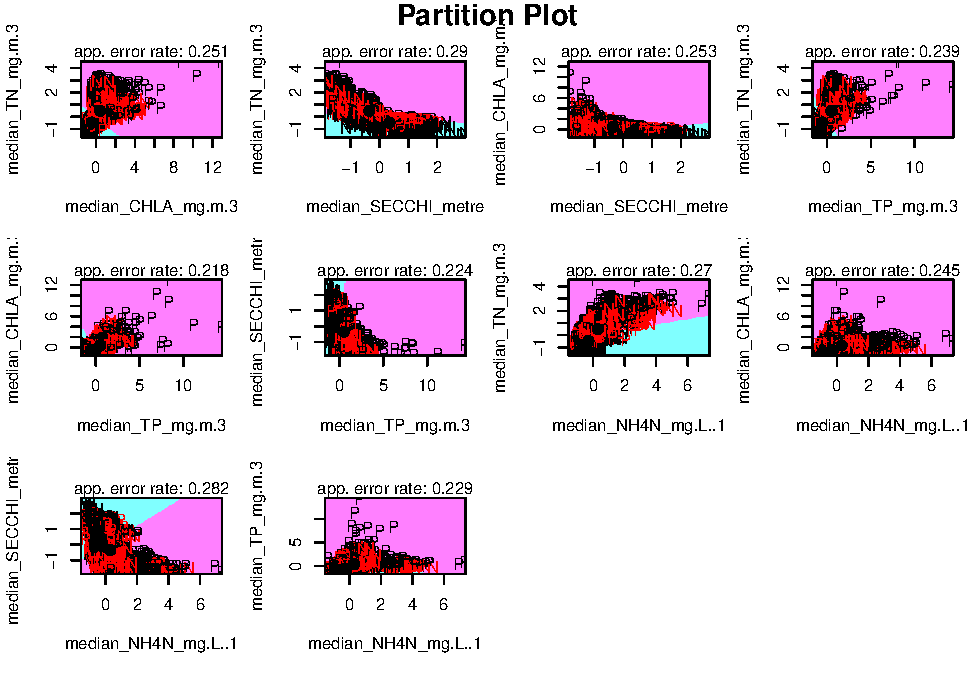
\includegraphics{Final-Report_files/figure-latex/unnamed-chunk-6-1.pdf}

The Partition plot while not any easier to interpret, sorted groups more appropriately and did not have unused partitions. We still see plenty of errors. The individual graphs give error rates between 0.218 and 0.29.

The accuracy was only slightly better at 76.7\%.

The implications of this LDA investigation suggest are that Dominant Landcover may be an indicator of the levels of lake health variables in a given lake. Therefore, if we know whether a lake has native or pastoral landcover, this could give us an indication on the health of a lake. It also means that in the case that the Dominant Landcover observation is lost for a lake, the value may be able to be imputed (with a note mentioning the imputation) with some level of accuracy by using the values from the Lake Health variables.

\hypertarget{discussion}{%
\subsection{Discussion}\label{discussion}}

\begin{itemize}
\tightlist
\item
  WHAT DOES IT MEEEAAAAAANNNNNNN
\item
  problems

  \begin{itemize}
  \tightlist
  \item
    clarity (not always possible as you may just have a shallow lake).
  \end{itemize}
\end{itemize}

\hypertarget{bibliography}{%
\subsection{Bibliography}\label{bibliography}}

\begin{itemize}
\tightlist
\item
  I have some references from research into health variables and where data from
\item
  APA referencing
\end{itemize}

data: \url{https://www.stats.govt.nz/indicators/modelled-lake-water-quality/}

\end{document}
